
\de{ĐỀ THI GIỮA HỌC KỲ II NĂM HỌC 2022-2023}{THPT Thủ Đức}

\Opensolutionfile{ans}[ans/ans]
%Câu 1
\begin{ex}%[0T7B3-2]%[Dự án đề kiểm tra HKII NH22-23- Phạm Văn Long]%[THPT Thủ Đức]
	Nghiệm của phương trình $\sqrt{31x^2 + 57x +2} = 5x + 4$ là
	\choice
	{$x= \dfrac{2}{3}$ và $x=-\dfrac{7}{2}$}
	{$x=-\dfrac{7}{2}$}
	{\True $x=\dfrac{2}{3}$}
	{$x=-\dfrac{2}{3}$}
	\loigiai{
		Ta có
		\allowdisplaybreaks
		\begin{eqnarray*}
		\sqrt{31x^2 + 57x + 2} = 5x + 4 
		&\Rightarrow & 31x^2 + 57x + 2 = 25x^2 + 40x + 16 \\
		&\Rightarrow & 6x^2 + 17x -14 = 0\\
		&\Rightarrow & \hoac{& x= \dfrac{2}{3}\\& x = -\dfrac{7}{2}.}
		\end{eqnarray*}
		Thử lại, ta thấy $x=\dfrac{2}{3}$ thỏa mãn.\\
		Vậy $S=\left\{\dfrac{2}{3}\right\}$.
	}
\end{ex}

%Câu 2
\begin{ex}%[0T7B1-2]%[Dự án đề kiểm tra HKII NH22-23- Phạm Văn Long]%[THPT Thủ Đức]
	Cho tam thức bậc hai $f(x)= -2x^2 + 8x -8$. Trong các mệnh đề sau, mệnh đề nào đúng?
	\choice
	{$f(x)>0$ với mọi $x\in \mathbb{R}$}
	{$f(x)\geq0$ với mọi $x\in \mathbb{R}$}
	{$f(x)<0$ với mọi $x\in \mathbb{R}$}
	{\True $f(x)\leq0$ với mọi $x\in \mathbb{R}$}
	\loigiai{
		Ta có $\heva{&a=-2 <0\\&\Delta = 8^2 -4\cdot (-2)\cdot(-8)= 0.}$
		Suy ra $f(x)\leq 0,\,\forall x\in \mathbb{R}$.
	}
\end{ex}

%Câu 3
\begin{ex}% [0T9B1-6] %[Dự án đề kiểm tra HKII NH22-23- Phạm Văn Long]%[THPT Thủ Đức]
	Trong mặt phẳng $Oxy$, cho hai véc-tơ $\overrightarrow{a} = \left(\sqrt{3};-15\right)$ và $\overrightarrow{b} = (-4;\sqrt{3})$. Góc giữa hai véc-tơ $\overrightarrow{a}$ và $\overrightarrow{b}$ bằng
	\choice
	{\True $120^\circ$}
	{$30^\circ$}
	{$60^\circ$}
	{$150^\circ$}
	\loigiai{
		Ta có 
		\[\cos \left(\overrightarrow{a},\overrightarrow{b}\right)=\dfrac{\overrightarrow{a}\cdot \overrightarrow{b}}{\left|\overrightarrow{a}\right|\cdot \left|\overrightarrow{b}\right|}=\dfrac{\sqrt{3}\cdot (-4) + (-15)\cdot\sqrt{3}}{\sqrt{\left(\sqrt{3}\right)^2 + (-15)^2}\cdot \sqrt{(-4)^2 + (\sqrt{3})^2}}=-\dfrac{1}{2}.\]
		 $\Rightarrow \left(\overrightarrow{a},\overrightarrow{b}\right)=120^\circ$
	}
\end{ex}

%Câu 4
\begin{ex}%[0T9B1-3]%[Dự án đề kiểm tra HKII NH22-23- Phạm Văn Long]%[THPT Thủ Đức]
	Trong mặt phẳng tọa độ $Oxy$, tìm tọa độ của $M'$ là điểm đối xứng của điểm $M(-3;6)$ qua trục $Oy$.
	\choice
	{$M'(-3;-6)$}
	{$M'(0;-6)$}
	{\True $M'(3;6)$}
	{$M'(3;0)$}
	\loigiai{
		Vì $M'$ đối xứng với $M$ qua $Oy$ nên ta có $\heva{&x_{M'}=-x_M = 3\\&y_{M'}=y_M=6.}$\\
		Vậy tọa độ của $M'$ là $M'(3;6).$
	}
\end{ex}

%Câu 5
\begin{ex}%[0T7B1-2]%[Dự án đề kiểm tra HKII NH22-23- Phạm Văn Long]%[THPT Thủ Đức]
	Cho tam thức bậc hai $f(x) = ax^2 + bx + c$ có bảng xét dấu như hình
	\begin{center}
		
\begin{tikzpicture}
			\tkzTabInit[nocadre=false,lgt=1.2,espcl=2,deltacl=.6]
			{$x$/0.8,$f(x)$/0.8}
			{$-\infty$,$-2$,$1$,$+\infty$}
			\tkzTabLine{,+,0,-,0,+,}
		\end{tikzpicture}
	\end{center}
	Mệnh đề nào sau đây \textbf{sai}?
	\choice
	{$f(-1)<0$}
	{\True $f(-1-\sqrt{2})> 0$}
	{$f(\pi) > 0$}
	{$f(-1+\sqrt{2})>0$}
	\loigiai{
		Từ bảng xét dấu, ta có mệnh đề sai là $f(-1+\sqrt{2})>0$.
	}
\end{ex}

%Câu 6
\begin{ex}%[0T9B1-3]%[Dự án đề kiểm tra HKII NH22-23- Phạm Văn Long]%[THPT Thủ Đức]
	Trong mặt phẳng $Oxy$, cho hai điểm $A(5;-2)$ và $B(-3;8)$. Tìm tọa độ trung điểm $I$ của đoạn thẳng $AB$.
	\choice
	{$I(-8;10)$}
	{$I(4;5)$}
	{\True $I(1;3)$}
	{$I(-4;5)$}
	\loigiai{
		Tọa độ trung điểm $I$ của đoạn thẳng $AB$ là $(1;3)$.
	}
\end{ex}

%Câu 7
\begin{ex}% [0T7B2-1]%[Dự án đề kiểm tra HKII NH22-23- Phạm Văn Long]%[THPT Thủ Đức]
	Tập nghiệm của bất phương trình $-3x^2 - 3x+ 18 <0 $ là
	\choice
	{$(-2;3)$}
	{\True $(-\infty;-3)\cup (2;+\infty)$}
	{$(-\infty;-2)\cup (3;+ \infty)$}
	{$(-3;2)$}
	\loigiai{
		Đặt $f(x)=-3x^2 -3x + 18$.\\
		Ta có $-3x^2 - 3x + 18=0 \Leftrightarrow \hoac{&x =2\\&x=-3.}$
		Bảng xét dấu
		\begin{center}
		
\begin{tikzpicture}
			\tkzTabInit[nocadre=false,lgt=1.2,espcl=2,deltacl=.6]
			{$x$/0.8,$f(x)$/0.8}
			{$-\infty$,$-3$,$2$,$+\infty$}
			\tkzTabLine{,-,0,+,0,-,}
		\end{tikzpicture}
		\end{center}
		Từ bảng xét dấu, ta có tập nghiệm của bất phương trình đã cho là $S=(-\infty;-3)\cup (2;+\infty)$.
	}
\end{ex}

%Câu 8
\begin{ex}% [0T7B2-1]%[Dự án đề kiểm tra HKII NH22-23- Phạm Văn Long]%[THPT Thủ Đức]
	\immini{
	Cho hàm số $f(x)=ax^2 + bx + c$ có đồ thị như hình bên. Tìm tập nghiệm của bất phương trình $ax^2 + bx + c\leq 0$. 
	\choice
	{$[0;3]$}
	{$\left(-\infty;-3\right)\cup (2;+\infty)$}
	{\True $(-\infty;-3] \cup [2;+\infty)$}
	{$[-3;2]$}
	}
	{
		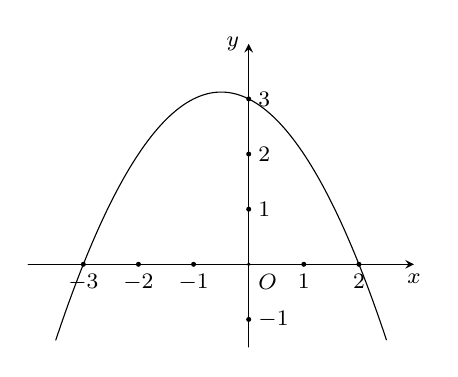
\begin{tikzpicture}[>=stealth,line join=round,line cap=round,font=\footnotesize,scale=0.7]
			\draw[->] (-4,0)--(3,0) node[below]{$x$};
			\draw[->] (0,-1.5)--(0,4) node[left]{$y$};
			\fill[name=O] (0,0) circle (1pt) node[below right] {$O$}; 
			\draw[color=black, smooth, samples=100, domain= -3.5:2.5] plot(\x,{-1/2*(\x + 3)*(\x -2)}) node[left]{$ $};
			\foreach \x in {-3,-2,-1,1,2}
				\fill (\x,0) circle (1.3pt)node[below]{$\x$};
			\foreach \y in {-1,1,2,3}
				\fill (0,\y) circle (1.3pt)node[right]{$\y$};
		\end{tikzpicture}
	}
	\loigiai{
		Từ đồ thị, ta có $f(x)\leq 0 \Leftrightarrow x\in (-\infty;-3]\cup [2;+\infty)$.
	}
\end{ex}

%Câu 9
\begin{ex}%[0T7B1-2]%[Dự án đề kiểm tra HKII NH22-23- Phạm Văn Long]%[THPT Thủ Đức]
	\immini{
	Cho hàm số bậc hai $f(x) = ax^2 + bx +c$ có đồ thị như hình vẽ. Đặt $\Delta = b^2 - 4ac$. Ta có
	\choice
	{$\heva{&a > 0 \\&\Delta \geq 0}$}
	{$\heva{&a > 0 \\&\Delta = 0}$}
	{$\heva{&a > 0 \\&\Delta < 0}$}
	{\True $\heva{&a > 0 \\&\Delta \leq 0}$}
	}
	{
		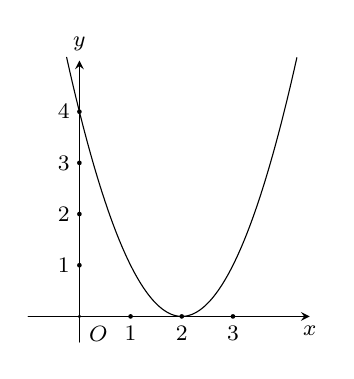
\begin{tikzpicture}[>=stealth,line join=round,line cap=round,font=\footnotesize,scale=0.65]
			\draw[->] (-1,0)--(4.5,0) node[below]{$x$};
			\draw[->] (0,-0.5)--(0,5) node[above]{$y$};
			\fill[name=O] (0,0) circle (1pt) node[below right] {$O$}; 
			\draw[color=black, smooth, samples=100, domain= -0.25:4.25] plot(\x,{(\x-2)^2}) node[left]{$ $};
			\foreach \x in {1,2,3}
				\fill (\x,0) circle (1.3pt)node[below]{$\x$};
			\foreach \y in {1,2,3,4}
				\fill (0,\y) circle (1.3pt)node[left]{$\y$};
		\end{tikzpicture}
	}
	\loigiai{
		Từ đồ thị ta thấy $f(x)\geq 0,\,\forall x \in \mathbb{R}$. Khi đó $\heva{&a>0 \\& \Delta \leq 0.}$
	}
\end{ex}

%Câu 10
\begin{ex}%[0T9B1-3] %[Dự án đề kiểm tra HKII NH22-23- Phạm Văn Long]%[THPT Thủ Đức]
	Trong mặt phẳng $Oxy$, cho $\triangle ABC$ có $A(1;3)$, $B(-4;2)$, $C(0;4)$. Tọa độ trọng tâm $G$ của $\triangle ABC$ là
	\choice
	{$(1;-3)$}
	{$(-1;3)$}
	{$(1;3)$}
	{$(-1;-3)$}
	\loigiai{
		Vì $G$ là trọng tâm của $\triangle ABC$ nên $\heva{&x_G = \dfrac{x_A + x_B + x_C}{3}=-1\\&y_G = \dfrac{y_A + y_B + y_C}{3}=3.}$\\
		Vậy tọa độ trọng tâm $G$ là $G(-1;3)$.
	}
\end{ex}

%Câu 11
\begin{ex}%[0T7B3-1]%[Dự án đề kiểm tra HKII NH22-23- Phạm Văn Long]%[THPT Thủ Đức]
	Số nghiệm của phương trình $\sqrt{2x^2 - 4x +2} = \sqrt{1-x}$ là
	\choice
	{\True $2$}
	{$0$}
	{$1$}
	{Vô số}
	\loigiai{
		Ta có
		\allowdisplaybreaks
		\begin{eqnarray*}
		\sqrt{2x^2 - 4x + 2} = \sqrt{1-x} 
		&\Rightarrow & 2x^2 - 4x + 2 = 1-x \\
		&\Rightarrow & 2x^2 - 3x + 1 = 0 \\
		&\Rightarrow & \hoac{&x = 1 \\&x = \dfrac{1}{2}}
		\end{eqnarray*}
		Thử lại, ta nhận $x=1$, $x=\dfrac{1}{2}$.\\
		Vậy tập nghiệm của phương trình là $S=\left\{1;\dfrac{1}{2}\right\}$.
	}
\end{ex}

%Câu 12
\begin{ex}%[0T7B1-2]%[Dự án đề kiểm tra HKII NH22-23- Phạm Văn Long]%[THPT Thủ Đức]
	\immini{
	Cho hàm số bậc hai $f(x) = ax^2 + bx + c$ có đồ thị như hình vẽ. Khẳng định nào dưới đây đúng?
	\choice
	{$f(x)>0 \Leftrightarrow x > 0$}
	{$f(x)>0 \Leftrightarrow 0 < x < 2$}
	{\True $f(x)>0 \Leftrightarrow \hoac{&x<1 \\ &x>2}$}
	{$f(x)>0 \Leftrightarrow 1 < x < 2$}
	}{
	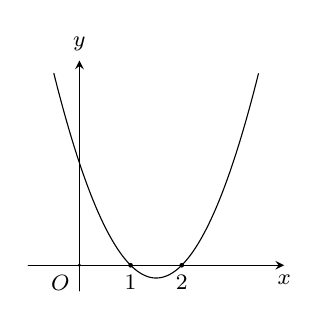
\begin{tikzpicture}[>=stealth,line join=round,line cap=round,font=\footnotesize,scale=0.65]
		\draw[->] (-1,0)--(4,0) node[below]{$x$};
		\draw[->] (0,-0.5)--(0,4) node[above]{$y$};
		\fill[name=O] (0,0) circle (1pt) node[below left] {$O$}; 
		\draw[color=black, smooth, samples=100, domain= -0.5:3.5] plot(\x,{(\x-2)*(\x-1)}) node[left]{$ $};
		\foreach \x in {1,2}
			\fill (\x,0) circle (1.3pt)node[below]{$\x$};
		% \foreach \y in {1,2,3,4}
		% 	\fill (0,\y) circle (1.3pt)node[left]{$\y$};
	\end{tikzpicture}
	}
	\loigiai{
		Từ đồ thị ta có $f(x) < 0 \Leftrightarrow 1<x <2$ và $f(x)>0 \Leftrightarrow \hoac{&x>2\\&x<1.}$
	}
\end{ex}

%Câu 13
\begin{ex}% [0T7K3-2]%[Dự án đề kiểm tra HKII NH22-23- Phạm Văn Long]%[THPT Thủ Đức]
	Nghiệm của phương trình $\sqrt{x + 1} = x$ có dạng $\dfrac{a+\sqrt{5}}{b}$ với $a$, $b \in \mathbb{N}^{*}$. Khi đó $a+b$ bằng
	\choice
	{$2$}
	{$5$}	
	{\True $3$}
	{$1$}
	\loigiai{
		Ta có 
		\allowdisplaybreaks
		\begin{eqnarray*}
		\sqrt{x+1} = x 
		&\Rightarrow & x + 1 = x^2 \\
		&\Rightarrow & x^2 -x -1 = 0 \\
		&\Rightarrow & \hoac{&x=\dfrac{1+\sqrt{5}}{2}\\& x= \dfrac{1-\sqrt{5}}{2}.}
		\end{eqnarray*}
		Thử lại, ta nhận $x=\dfrac{1+\sqrt{5}}{2}$.\\
		Vậy $a = 1$, $b= 2$ và $a+b = 3$.
	}
\end{ex}

%Câu 14
\begin{ex}% [0T9Y2-2]%[Dự án đề kiểm tra HKII NH22-23- Phạm Văn Long]%[THPT Thủ Đức]
	Trong mặt phẳng $Oxy$, đường thẳng đi qua $A(-1;7)$, nhận $\overrightarrow{n}=(-2;4)$ làm véc-tơ pháp tuyến có phương trình là
	\choice
	{$-x+2y+15=0$}
	{$-2x+4y+26=0$}
	{\True $x-2y+15=0$}
	{$x+y-6=0$}
	\loigiai{
		Đường thẳng qua $A(-1;7)$, nhận $\overrightarrow{n}=(-2;4)$ có phương trình
		\[-2(x+1) + 4(y-7)=0 \Leftrightarrow -2x + 4y -30=0\Leftrightarrow x-2y+15=0.\]
	}
\end{ex}

%Câu 15
\begin{ex}%[0T7B1-2] V%[Dự án đề kiểm tra HKII NH22-23- Phạm Văn Long]%[THPT Thủ Đức]
	Trong tất cả các giá trị của tham số $m$ để phương trình $x^2 - 4x + 3m^2 -23m +14=0$ có 2 nghiệm trái dấu
	\choice
	{\True $\dfrac{3}{3} < m < 7$}
	{$\hoac{&m\geq 7\\& m\leq \dfrac{2}{3}}$}
	{$\hoac{&m>7\\&m<\dfrac{2}{2}}$}
	{$\dfrac{2}{3}\leq m \leq 7$}
	\loigiai{
		Ta có phương trình đã cho có hai nghiệm trái dấu khi $$ac<0\Leftrightarrow 3m^2 -23m+14<0\Leftrightarrow \dfrac{2}{3}<m<7.$$
	}
\end{ex}

%Câu 16
\begin{ex}%[0T7B1-4]%[Dự án đề kiểm tra HKII NH22-23- Phạm Văn Long]%[THPT Thủ Đức]
	Phương trình $(x+2)\sqrt{x-1}=0$
	\choice
	{\True có nghiệm duy nhất}
	{vô nghiệm}
	{có hai nghiệm trái dấu}
	{có hai nghiệm dương}
	\loigiai{
		Ta có
		\allowdisplaybreaks
		\begin{eqnarray*}
		(x+2)\sqrt{x-1}=0
		&\Rightarrow& \hoac{&x + 2=0\\&\sqrt{x-1}=0}\\
		&\Rightarrow& \hoac{&x=-2\\&x=1.}
		\end{eqnarray*}
		Thử lại, ta nhận $x=1$. Vậy phương trình đã cho có nghiệm duy nhất.
	}
\end{ex}

%Câu 17
\begin{ex}%[0T9B2-3]  %[Dự án đề kiểm tra HKII NH22-23- Phạm Văn Long]%[THPT Thủ Đức]
	Trong mặt phẳng $Oxy$, xác định vị trí tương đối của $2$ đường thẳng $\left(\Delta_1\right)\colon \dfrac{x}{2} - \dfrac{y}{3}=1$ và $\left(\Delta_2\right)\colon 6x-2y-8=0$.
	\choice
	{Trùng nhau}
	{\True Cắt nhau}
	{Song song}
	{Vuông góc với nhau}
	\loigiai{
		Ta có $\overrightarrow{n}_1 = \left(\dfrac{1}{2};-\dfrac{1}{3}\right)$, $\overrightarrow{n}_2=\left(6;-2\right)$.\\
		Vì $\dfrac{1}{2}\cdot (-2) \neq -\dfrac{1}{3}\cdot 6$ nên $\left(\Delta_1\right)$ cắt $\left(\Delta_2\right)$.
	}
\end{ex}

%Câu 18
\begin{ex}%[0T7B1-1]%[Dự án đề kiểm tra HKII NH22-23- Phạm Văn Long]%[THPT Thủ Đức]
	Tam thức bậc hai $f(x)$ nào có bảng xét dấu như hình bên dưới
	\begin{center}
		
\begin{tikzpicture}
			\tkzTabInit[nocadre=false,lgt=1.2,espcl=2,deltacl=.6]
			{$x$/0.8,$f(x)$/0.8}
			{$-\infty$,$-7$,$6$,$+\infty$}
			\tkzTabLine{,-,0,+,0,-,}
		\end{tikzpicture}
	\end{center}
	\choice
	{$f(x) = -2x^2 + 2x + 84$}
	{$f(x) = x^2 + x -42$}
	{$f(x) = x^2 - x -42$}
	{\True $f(x) = -\dfrac{1}{2}x^2 - \dfrac{1}{2}x + 21$}
	\loigiai{
		Bảng xét dấu trên là của tam thức bậc hai $f(x)=-\dfrac{1}{2}x^2 -\dfrac{1}{2}x + 21$.
	}
\end{ex}

%Câu 19
\begin{ex}%[0T7B1-1]%[Dự án đề kiểm tra HKII NH22-23- Phạm Văn Long]%[THPT Thủ Đức]
	Biểu thức nào sau đây là tam thức bậc hai?
	\choice
	{$f(x) = 2x - 4$}
	{$f(x) = \dfrac{1}{x} + 2x - 1$}
	{\True $f(x) = \dfrac{3x^2 + 2x - 6}{2}$}
	{$f(x) = x^4 - 2x^2 + 1$}
	\loigiai{
		Biểu thức bậc hai là $f(x)=\dfrac{3x^2 + 2x - 6}{2}$.
	}
\end{ex}

%Câu 20
\begin{ex}% [0T9B1-3] %[Dự án đề kiểm tra HKII NH22-23- Phạm Văn Long]%[THPT Thủ Đức]
	Trong mặt phẳng $Oxy$, cho $3$ điểm $M(-1;3)$, $N(2;0)$, $P(6;2)$. Tìm tọa độ $Q$ sao cho tứ giác $MNPQ$ là hình bình hành.
	\choice
	{$(9;-1)$}
	{\True $(3;5)$}
	{$(-1;9)$}
	{$(5;3)$}
	\loigiai{
		Ta có tứ giác $MNPQ$ là hình bình hành khi
		\[\overrightarrow{MN} = \overrightarrow{QP} \Leftrightarrow \heva{&x_N - x_M = x_P - x_Q\\&y_N - y_M = y_P - y_Q}\Leftrightarrow \heva{&2-(-1)=6-x_Q\\&0-3=2-y_Q}\Leftrightarrow \heva{&x_Q = 3\\&y_Q=5.}\]
		Vậy tọa độ điểm $Q$ là $Q(3;5)$.
	}
\end{ex}


\begin{ex}%[0H9Y2-1]%[Dự án đề kiểm tra GHKII NH22-23-Don Lee]%[Thủ Đức]
	Trong mặt phẳng $Oxy$, cho phương trình đường thẳng $d\colon 3x-2y+10=0$. Một véc-tơ pháp tuyến của đường thẳng $d$ là
	\choice
	{$\vec{n}=(6; 9)$}
	{\True $\vec{n}=(3;-2)$}
	{$\vec{n}=(3; 2)$}
	{$\vec{n}=(9; 6)$}
	\loigiai{
		Một véc-tơ pháp tuyến của đường thẳng $d$ là $\vec{n}=(3;-2)$.
	}
\end{ex}

\begin{ex}%[0D7B2-1]%[Dự án đề kiểm tra GHKII NH22-23-Don Lee]%[Thủ Đức]
	Bất phương trình $x^2+3x-4\leq 0$ có tất cả bao nhiêu nghiệm nguyên dương?
	\choice
	{$4$}
	{$3$}
	{$2$}
	{\True $1$}
	\loigiai{
		Ta có $x^2+3x-4\leq 0 \Leftrightarrow -4\le x\le 1$.\\
		Mà $x\in \mathbb{N}^*$ suy ra $x\in \{1\}$.\\
		Vậy phương trình đã cho có $1$ nghiệm nguyên dương.
	}
\end{ex}

\begin{ex}%[0D7B2-2]%[Dự án đề kiểm tra GHKII NH22-23-Don Lee]%[Thủ Đức]
	Biết rằng tập nghiệm của bất phương trình $\dfrac{x^2-3x-28}{x^2-16}\leq 0$ là $S=(a; b]$. Tìm giá trị của $T=b-2a$.
	\choice
	{\True $T=-1$}
	{$T=15$}
	{$T=12$}
	{$T=-4$}
	\loigiai{
		Ta có
		\begin{itemize}
			\item $x^2-3x-28=0 \Leftrightarrow x=-4; x=7$.
			\item $x^2-16=0 \Leftrightarrow x=-4; x=4$.
		\end{itemize}
		Bảng xét dấu
		\begin{center}
			
\begin{tikzpicture}
				\tkzTabInit[nocadre=true,lgt=3,espcl=2,deltacl=0.5]
				{$x$/0.8 , $x^2-3x-18$/0.8 , $x^2-16$/0.8 , VT/0.8}
				{$-\infty$,$-4$,$4$,$7$,$+\infty$}
				\tkzTabLine{,+,0,-,t,-,0,+,}
				\tkzTabLine{,+,0,-,0,+,t,+,}
				\tkzTabLine{,+,d,+,d,-,0,+,}
			\end{tikzpicture}
		\end{center}
		Dựa vào bảng xét dấu, ta có tập nghiệm của bất phương trình $\dfrac{x^2-3x-28}{x^2-16}\leq 0$ là $S=(4; 7]$.\\
		Giá trị của $T=b-2a=-1$.
	}
\end{ex}

\begin{ex}%[0D7B3-2]%[Dự án đề kiểm tra GHKII NH22-23-Don Lee]%[Thủ Đức]
	Kết luận nào sau đây đúng với phương trình $\sqrt{5x^2-28x-29}=\sqrt{x^2-5x+6}$?
	\choice
	{Phương trình có hai nghiệm phân biệt cùng dương}
	{Phương trình vô nghiệm}
	{Phương trình có hai nghiệm phân biệt cùng âm}
	{\True Phương trình có hai nghiệm trái dấu}
	\loigiai{
		Ta có\\
		\allowdisplaybreaks
		$\begin{aligned}[t]
			\sqrt{5x^2-28x-29}=\sqrt{x^2-5x+6}&\Leftrightarrow \heva{&x^2-5x+6\ge 0\\&5x^2-28x-29=x^2-5x+6}\\
			&\Leftrightarrow \heva{&x\le 2; x\ge 3\\&4x^2-23x-35=0}\\
			&\Leftrightarrow \heva{&x\le 2; x\ge 3\\&x=-\dfrac{5}{4}; x=7}\\
			&\Leftrightarrow x=-\dfrac{5}{4}; x=7.
		\end{aligned}$\\
		Vậy phương trình có hai nghiệm trái dấu.
	}
\end{ex}

\begin{ex}%[0H9Y1-3]%[Dự án đề kiểm tra GHKII NH22-23-Don Lee]%[Thủ Đức]
	Trong mặt phằng tọa độ $(O, \vec{i}, \vec{j})$, cho véc-tơ $\vec{u}=\vec{j}-3\vec{i}$. Khẳng định nào sau đây đúng?
	\choice
	{$\vec{u}=(1;-3)$}
	{$\vec{u}=(\vec{j}; -3\vec{i})$}
	{\True $\vec{u}=(-3; 1)$}
	{$\vec{u}=(-3\vec{i}; \vec{j})$}
	\loigiai{
		Có $\vec{u}=\vec{j}-3\vec{i}$ suy ra $\vec{u}=(-3; 1)$.
	}
\end{ex}

\begin{ex}%[0D7Y2-1]%[Dự án đề kiểm tra GHKII NH22-23-Don Lee]%[Thủ Đức]
	Trong các bất phương trình sau, bất phương trình nào không là bất phương trình bậc hai một ẩn?
	\choice
	{$a^2+2a+3<0$}
	{$x^2-2x\left(\dfrac{1}{x}-x\right)<1$}
	{\True $2x^2-\sqrt{3}x>0$}
	{$3y^2+5y+7\leq 0$}
	\loigiai{
		Bất phương trình $2x^2-\sqrt{3}x>0$ không là bất phương trình bậc hai một ẩn.
	}
\end{ex}

\begin{ex}%[0D7B2-1]%[Dự án đề kiểm tra GHKII NH22-23-Don Lee]%[Thủ Đức]
	Bất phương trình nào sau đây có một nghiệm duy nhất?
	\choice
	{\True $4x^2-12x+9\leq 0$}
	{$-9x^2+6x-1\leq 0$}
	{$-x^2-x+2>0$}
	{$x^2-2x+1\geq 0$}
	\loigiai{
		Ta có $4x^2-12x+9\leq 0 \Leftrightarrow (2x-3)^2 \le 0 \Leftrightarrow 2x-3=0 \Leftrightarrow x=\dfrac{3}{2}$.
	}
\end{ex}

\begin{ex}%[0D7B3-2]%[Dự án đề kiểm tra GHKII NH22-23-Don Lee]%[Thủ Đức]
	Tập nghiệm của phương trình $\sqrt{3x^2-2x}=\sqrt{x^2+x-1}$ là 
	\choice
	{$S=\varnothing$}
	{$S=\left\{\dfrac{1}{2}\right\}$}
	{$S=\left\{1; \dfrac{1}{2}\right\}$}
	{\True $S=\{1\}$}
	\loigiai{
		Ta có\\
		\allowdisplaybreaks
		$\begin{aligned}[t]
			\sqrt{3x^2-2x}=\sqrt{x^2+x-1}&\Leftrightarrow \heva{&3x^2-2x\ge 0\\&3x^2-2x=x^2+x-1}\\
			&\Leftrightarrow \heva{&x\le 0; x\ge \dfrac{2}{3}\\&2x^2-3x+1=0}\\
			&\Leftrightarrow \heva{&x\le 0; x\ge \dfrac{2}{3}\\&x=\dfrac{1}{2}; x=1}\\
			&\Leftrightarrow x=1.
		\end{aligned}$\\
		Vậy phương trình có tập nghiệm $S=\{1\}$.
	}
\end{ex}

\begin{ex}%[0H9B2-5]%[Dự án đề kiểm tra GHKII NH22-23-Don Lee]%[Thủ Đức]
	Trong mặt phẳng $Oxy$, khoảng cách từ điểm $M(15; 1)$ đến đường thẳng $\Delta\colon x-3y-2=0$ là
	\choice
	{\True $\sqrt{10}$}
	{$\dfrac{16}{\sqrt{5}}$}
	{$\dfrac{1}{\sqrt{10}}$}
	{$\sqrt{5}$}
	\loigiai{
		Ta có $\mathrm{d}\left(M, \Delta\right)=\dfrac{|15-3\cdot 1-2|}{\sqrt{1^2+(-3)^2}}=\sqrt{10}$.
	}
\end{ex}

\begin{ex}%[0H9Y2-1]%[Dự án đề kiểm tra GHKII NH22-23-Don Lee]%[Thủ Đức]
	Trong mặt phẳng $Oxy$, một véc-tơ chỉ phương của đường thẳng $d\colon \heva{&x=1-t\\&y=-2+6t}, (t\in \mathbb{R})$ là
	\choice
	{$\vec{u}=(1;-2)$}
	{$\vec{u}=(1; 6)$}
	{$\vec{u}=(6; 1)$}
	{\True $\vec{u}=(1;-6)$}
	\loigiai{
		Một véc-tơ chỉ phương của đường thẳng $d$ là $\vec{u}=(1;-6)$.
	}
\end{ex}

\begin{ex}%[0H9B2-2]%[Dự án đề kiểm tra GHKII NH22-23-Don Lee]%[Thủ Đức]
	Trong mặt phẳng $Oxy$, viết phương trình tham số của đường thẳng đi qua hai điểm $A(-2; 5)$ và $B(2;-1)$.
	\choice
	{$\heva{&x=-2-4t\\&y=-1-6t}\,\, (t\in \mathbb{R})$}
	{\True $\heva{&x=-2+2t\\&y=5-3t}\,\, (t\in \mathbb{R})$}
	{$\heva{&x=2+4t\\&y=5-6t}\,\, (t\in \mathbb{R})$}
	{$\heva{&x=-2+6t\\&y=5+4t}\,\, (t\in \mathbb{R})$}
	\loigiai{
		Ta có $\overrightarrow{AB}=(4; -6)$, chọn $\vec{u}=(2; -3)$ là véc-tơ chỉ phương của $AB$.\\
		Phương trình của đường thẳng $AB\colon \heva{&x=-2+2t\\&y=5-3t}\,\, (t\in \mathbb{R})$.
	}
\end{ex}

\begin{ex}%[0H9B2-4]%[Dự án đề kiểm tra GHKII NH22-23-Don Lee]%[Thủ Đức]
	Trong mặt phẳng $Oxy$, góc giữa $2$ đường thẳng $\Delta_1\colon x+2y-7=0$ và $\Delta_2\colon \heva{&x=t\\&y=100+2t}\,\,(t\in \mathbb{R})$ là
	\choice
	{$60^{\circ}$}
	{\True $90^{\circ}$}
	{$120^{\circ}$}
	{$30^{\circ}$}
	\loigiai{
		Đường thẳng $\Delta_1$, $\Delta_2$ có véc-tơ pháp tuyến lần lượt là $\vec{n}_1=(1; 2)$, $\vec{n}_2=(2; -1)$.\\
		Ta có $\vec{n}_1\cdot \vec{n}_2=0$ suy ra $\Delta_1 \perp \Delta_2$. Vậy góc giữa $2$ đường thẳng $\Delta_1$ và $\Delta_2$ là $90^{\circ}$.
	}
\end{ex}

\begin{ex}%[0D3B2-4]%[Dự án đề kiểm tra GHKII NH22-23-Don Lee]%[Thủ Đức]
	\immini
	{Cho đồ thị của hai hàm số bậc hai $f(x)=ax^2+bx+c$ và $g(x)=dx^2+ex+f$ như hình vẽ. Khẳng định nào đúng với phương trình $\sqrt{ax^2+bx+c}=\sqrt{dx^2+ex+f}$?
	\choice
	{Phương trình có nghiệm duy nhất là $x=\dfrac{3}{2}$}
	{\True Phương trình vô nghiệm}
	{Phương trình có nghiệm duy nhất là $x=0$}
	{Phương trình có $2$ nghiệm phân biệt là $x=0$ và $x=\dfrac{3}{2}$}}
	{\begin{tikzpicture}[x=1cm,y=1cm,scale=1]
			\draw[->] (-1.5,0)--(2.5,0)node[below right]{$x$};
			\draw[->] (0,-3.5)--(0,2)node[left]{$y$};
			\fill (0,0)node[below left]{$O$} circle(1pt);
			\fill (0,-2)node[left]{$-2$} circle(1pt);
			\fill (3/2,0)node[above]{\footnotesize $\dfrac{3}{2}$} circle(1pt);
			\fill (1.7,1.2)node[above]{$y=f(x)$};
			\fill (1.5,-3.5)node[above]{$y=g(x)$};
			\draw[black,samples=150,smooth,domain=-1.5:2.5] plot(\x,{(\x)^2-(\x)-2});
			\draw[black,samples=150,smooth,domain=-0.5:2.5] plot(\x,{-(\x)^2+2*(\x)-2});
			\draw[dashed] (3/2,0)--(3/2,-5/4);
	\end{tikzpicture}}
	\loigiai{
		Ta có $\sqrt{ax^2+bx+c}=\sqrt{dx^2+ex+f} \Leftrightarrow \heva{&ax^2+bx+c\ge 0\\&ax^2+bx+c=dx^2+ex+f}$.\\
		Số nghiệm của phương trình bằng số điểm chung thuộc trục $Ox$ hoặc nằm phía trên trục $Ox$ của hai đồ thị $f(x)=ax^2+bx+c$ và $g(x)=dx^2+ex+f$.\\
		Dựa vào đồ thị, ta có phương trình $\sqrt{ax^2+bx+c}=\sqrt{dx^2+ex+f}$ vô nghiệm.
	}
\end{ex}

\begin{ex}%[0D7T2-1]%[Dự án đề kiểm tra GHKII NH22-23-Don Lee]%[Thủ Đức]
	Một hòn đá được ném thẳng lên từ độ cao $3{,}4$ m so với mặt đất với vận tốc $10$ m/s. Độ cao của hòn đá so với mặt đất (tính bằng mét) sau $t$ giây được cho bời hàm số $h(t)=-4{,}9t^2+10t+3{,}4$. Hỏi hòn đá ở độ cao trên $5$ m trong khoảng thời gian bao lâu? Làm tròn kết quả đến hàng phần trăm.
	\choice
	{\True $1{,}69$ giây}
	{$1{,}71$ giây}
	{$1{,}67$ giây}
	{$1{,}73$ giây}
	\loigiai{
		Ta có $h(t)=-4{,}9t^2+10t+3{,}4 > 5 \Leftrightarrow -4{,}9t^2+10t-1{,}6 > 0$.\\
		Phương trình $-4{,}9t^2+10t-1{,}6=0$ có $\Delta'=5^2-(-4{,}9)\cdot(-1{,}6)=\dfrac{429}{25}>0$ nên có $2$ nghiệm $t_1<t_2$.\\
		Suy ra bất phương trình $-4{,}9t^2+10t-1{,}6 > 0$ có nghiệm $t_1<t<t_2$.\\
		Vậy khoảng thời gian hòn đá ở độ cao trên $5$ m là $t_2-t_1=\dfrac{2\sqrt{\Delta'}}{4{,}9}\approx 1{,}69$ giây.
	}
\end{ex}

\begin{ex}%[0H9B1-5]%[Dự án đề kiểm tra GHKII NH22-23-Don Lee]%[Thủ Đức]
	Trong mặt phẳng $Oxy$, cho ba điểm $A(2;-4)$, $B(6; 0)$, $C(m; 4)$. Tìm $m$ để $A$, $B$, $C$ thẳng hàng.
	\choice
	{\True $m=10$}
	{$m=-6$}
	{$m=2$}
	{$m=-10$}
	\loigiai{
		Ta có $\overrightarrow{AB}=(4; 4)$, $\overrightarrow{AC}=(m-2; 8)$.\\
		Ba điểm $A$, $B$, $C$ thẳng hàng khi $\overrightarrow{AB}$ và $\overrightarrow{AC}$ cùng phương $\Leftrightarrow \dfrac{m-2}{4}=\dfrac{8}{4} \Leftrightarrow m=10$.
	}
\end{ex}

\begin{ex}%[0D3B1-1]%[Dự án đề kiểm tra GHKII NH22-23-Don Lee]%[Thủ Đức]
	\immini
	{Để tham gia một phòng tập thể dục người tập phải tham gia một khoản phí tham gia ban đầu và phí sử dụng phòng tập. Đường thẳng $\Delta$ trong hình vẽ bên biểu thị tổng chi phí (đơn vị: triệu đồng) tham gia một phòng tập thể dục theo thời gian tập của một người (đơn vị: tháng). Tính tổng chi phí mà người đó phải trả khi tham gia phòng tập thể dục trong thời gian $1$ năm.
	\choice
	{$8,5$ triệu đồng}
	{$8$ triệu đồng}
	{\True $7$ triệu đồng}
	{$6,5$ triệu đồng}}
	{\begin{tikzpicture}[x=1cm,y=1cm,scale=1]
			\draw[->] (-0.5,0)--(5,0)node[below]{tháng};
			\draw[->] (0,-0.5)--(0,4)node[left]{tiền};
			\fill (0,0)node[below left]{$O$};
			\fill (0,1)node[left]{$1$};
			\fill (4,0)node[below]{$4$};
			\fill (0,3)node[left]{$3$};
			\fill (4.2,3.1)node[above]{$\Delta$};
			\draw[dashed] (0,3)--(4,3)--(4,0);
			\draw[black,samples=150,smooth,domain=0:4.5] plot(\x,{1/2*(\x)+1});
	\end{tikzpicture}}
	\loigiai{
		Dựa vào đồ thị, ta có $\Delta\colon y=f(x)=\dfrac{1}{2}x+1$.\\
		Tổng chi phí mà người đó phải trả khi tham gia phòng tập thể dục trong thời gian $1$ năm là $f(12)=7$ (triệu).
	}
\end{ex}

\begin{ex}%[0D7T2-1]%[Dự án đề kiểm tra GHKII NH22-23-Don Lee]%[Thủ Đức]
	Bác Tú có một tấm lưới thép gai dài $200$ m, bác cắt tấm lưới này thành $2$ đoạn là $x$ (m) và $200-x$ (m) để rào thành hai mảnh vườn hình vuông ở hai khu đất riêng biệt. Để tổng diện tích của $2$ mảnh vườn tối đa là $1700$ m$^2$ thì
	\choice
	{$40<x<160$}
	{$40<x<150$}
	{\True $40\leq x\leq 160$}
	{$39\leq x\leq 159$}
	\loigiai{
		Ta có $\left(\dfrac{x}{4}\right)^2+\left(\dfrac{200-x}{4}\right)^2\leq 1700 \Leftrightarrow x^2-200x+6400\le 0 \Leftrightarrow 40\le x\le 160$.
	}
\end{ex}

\begin{ex}%[0H9B1-4]%[Dự án đề kiểm tra GHKII NH22-23-Don Lee]%[Thủ Đức]
	Trong mặt phẳng $Oxy$, cho $2$ điểm $A(4;-2), B(10; 4)$ và điểm $M(x; 0)$ thỏa mãn $\left|\overrightarrow{MA}+\overrightarrow{MB}\right|$ có giá trị nhỏ nhất. Khẳng định nào sau đây đúng?
	\choice
	{$7<x<9$}
	{\True $6<x<8$}
	{$8<x<9$}
	{$0<x<7$}
	\loigiai{
		Gọi $I(7; 1)$ là trung điểm của $AB$.\\
		Ta có $\left|\overrightarrow{MA}+\overrightarrow{MB}\right|=2\left|\overrightarrow{MI}\right|=2IM=2\sqrt{(x-7)^2+(0-1)^2}\ge 2$.\\
		Dấu \lq\lq$=$\rq\rq\, xảy ra khi $x=7$.
	}
\end{ex}

\begin{ex}%[0D7B2-1]%[Dự án đề kiểm tra GHKII NH22-23-Don Lee]%[Thủ Đức]
	Cho biểu thức $f(x)=-x^2-7x+30$. Chọn phát biểu đúng.
	\choice
	{$f(0)<0$}
	{$f\left(3^{112}\right)>0$}
	{$f\left(-2^{2023}\right)>0$}
	{\True $f\left(2^{2023}\right)<0$}
	\loigiai{
		Xét $f(x)>0 \Leftrightarrow -x^2-7x+30>0 \Leftrightarrow -10<x<3$.\\
		Suy ra $f\left(2^{2023}\right)<0$.
	}
\end{ex}

\begin{ex}%[0D7B2-1]%[Dự án đề kiểm tra GHKII NH22-23-Don Lee]%[Thủ Đức]
	\immini
	{Cho đồ thị của hai hàm số bậc hai $y=f(x)$ và $y=g(x)$ như hình bên. Bất phương trình $f(x)\geq g(x)$ có tập nghiệm là
	\choice
	{$[0; 2]$}
	{\True $(-\infty; 0]\cup [2;+\infty)$}
	{$(-\infty; 1]\cup [2;+\infty)$}
	{$[0; 1]$}}
	{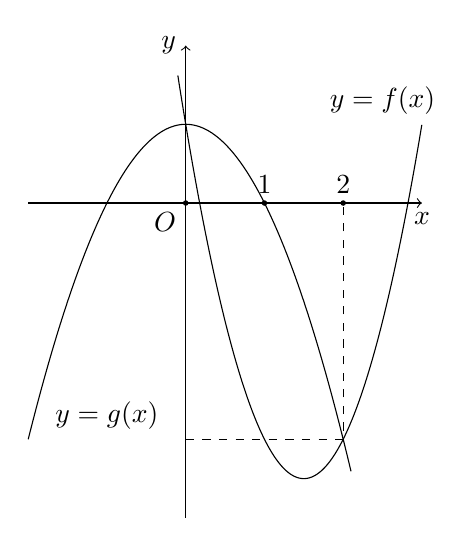
\begin{tikzpicture}[x=1cm,y=1cm,scale=1]
			\draw[->] (-2,0)--(3,0)node[below]{$x$};
			\draw[->] (0,-4)--(0,2)node[left]{$y$};
			\fill (0,0)node[below left]{$O$} circle(1pt);
			\fill (1,0)node[above]{$1$} circle(1pt);
			\fill (2,0)node[above]{$2$} circle(1pt);
			\fill (2.5,1)node[above]{$y=f(x)$};
			\fill (-1,-3)node[above]{$y=g(x)$};
			\draw[black,samples=150,smooth,domain=-2:2.1] plot(\x,{-(\x)^2+1});
			\draw[black,samples=150,smooth,domain=-0.1:3] plot(\x,{2*(\x)^2-6*(\x)+1});
			\draw[dashed] (0,-3)--(2,-3)--(2,0);
	\end{tikzpicture}}
	\loigiai{
		Tập nghiệm của bất phương trình $f(x)\geq g(x)$ là tập giá trị của $x$ sao cho đồ thị hàm số $y=f(x)$ nằm phía trên đồ thị hàm số $y=g(x)$ bao gồm cả các điểm chung của hai đồ thị.\\
		Dựa vào đồ thị, ta có tập nghiệm của bất phương trình $f(x)\geq g(x)$ là $(-\infty; 0]\cup [2;+\infty)$.
	}
\end{ex}

\Closesolutionfile{ans}
%\begin{center}
%	\textbf{ĐÁP ÁN}
%	\inputansbox{10}{ans/ans}	
%\end{center}
